\documentclass[10pt,a4paper]{article}
\usepackage[margin=2.2cm]{geometry}
\usepackage{fontspec}
\usepackage{kotex}
\setmainfont{Apple SD Gothic Neo}
\setsansfont{Apple SD Gothic Neo}
\usepackage{amsmath,amssymb}
\usepackage{graphicx}
\usepackage{booktabs}
\usepackage{caption}
\usepackage[dvipsnames]{xcolor}
\usepackage[colorlinks=true,linkcolor=MidnightBlue,citecolor=MidnightBlue,
            urlcolor=MidnightBlue]{hyperref}
\usepackage{titlesec}
\titleformat{\section}{\large\bfseries}{\thesection}{0.6em}{}
\titleformat{\subsection}{\normalsize\bfseries}{\thesubsection}{0.5em}{}
\captionsetup{font=small,labelfont=bf}
\setlength{\parskip}{0.35em}
\setlength{\parindent}{0pt}

\usepackage{mdframed}
\newmdenv[linewidth=0.4pt,linecolor=gray!60,backgroundcolor=gray!5,
          innertopmargin=6pt,innerbottommargin=6pt,skipabove=8pt,skipbelow=8pt]{claimbox}
\newcommand{\claim}[2]{\begin{claimbox}\textbf{주장.} #1\par\smallskip
  \textcolor{gray!70}{\textbf{반증 조건.} #2}\end{claimbox}}

\title{\bfseries 형태가 살아남았다\\[2pt]
\large 바닥에도 뽑기 여섯 --- 그리고 6연속 적중이 끊긴 이유}
\author{월드모델 실험실 · 노트 $814$}
\date{2026-08-07}
\begin{document}\maketitle

\section{한 줄}

논문 $175$ 가 판정 없이 남긴 후보를, 이번엔 \textbf{갈래 번호 우선순위}(규약
$46$ · 첫 이행)를 박고 판정했다 --- 안정 무리 세 쌍의 곡선 형태.

\begin{center}
\begin{tabular}{lrrrl}
\toprule
쌍 & 쌍 RMSE & 쌍 바닥($10$회) & 영분포 p$95$ & 판정 \\
\midrule
게임-모바일 & $0.0864$ & $0.1308$ & $0.0511$ & \textbf{2.같다}($0.66\times$) \\
모바일-세계애니 & $0.1584$ & $0.1404$ & $0.2324$ & \textbf{2.같다}($1.13\times$) \\
게임-세계애니 & $0.1864$ & $0.0681$ & $0.1954$ & \textbf{3.모른다}($2.7\times$) \\
\bottomrule
\end{tabular}
\end{center}

\textbf{(다르다)가 하나도 없다.} 두 쌍은 잡음 안에서 같고, 가장 날카로운
쌍(게임-세계애니)은 $2.7$배인데 합동 영분포(불균형 $146$ 대 $1{,}114$ 라
넓다)를 못 넘어 검정력 부족이다. \textbf{사용자의 인수분해 가설(공유 형태
$\times$ 도메인 모수)이 안정 무리에서 기각되지 않았다} --- 확정도 아니다.
판정력은 KOBIS(진폭 클 네 번째 안정 도메인)가 준다.

\begin{figure}[t]\centering
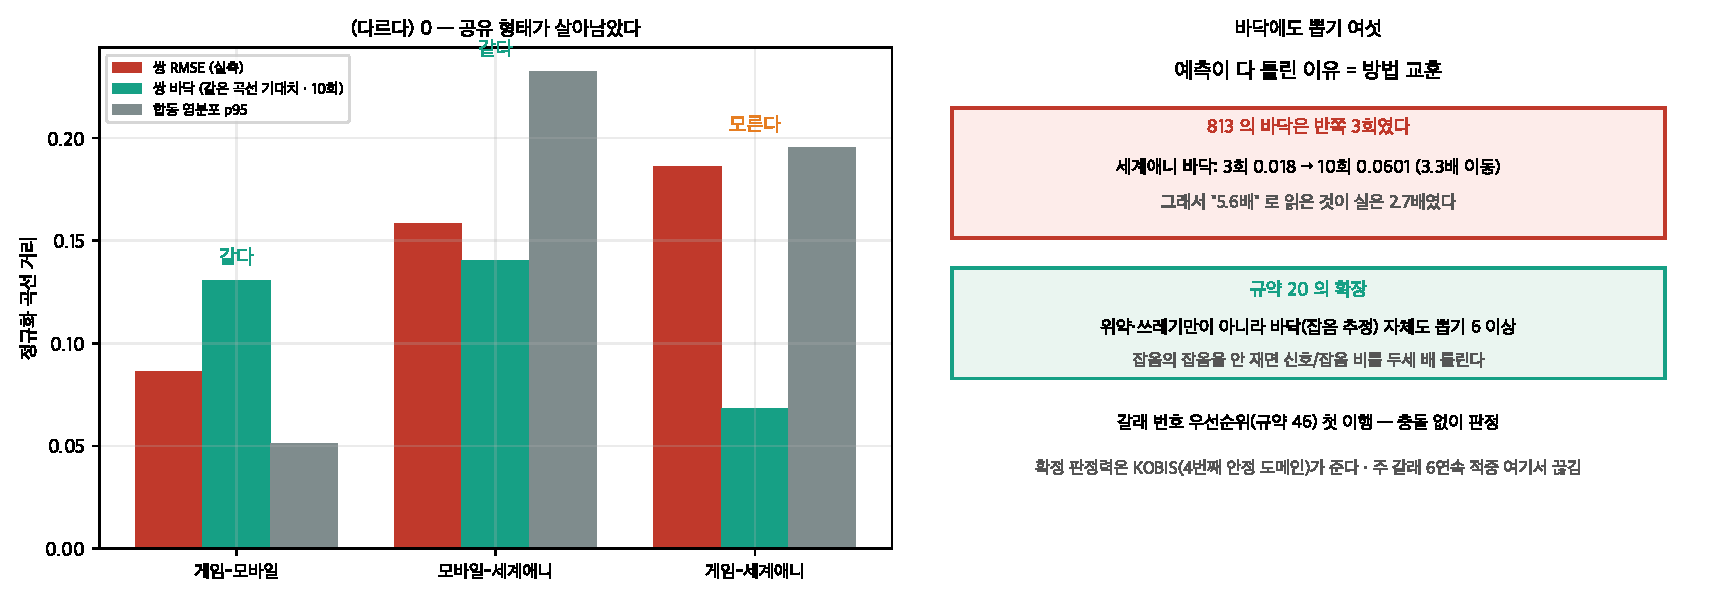
\includegraphics[width=0.95\textwidth]{figs/shape.pdf}
\caption{왼쪽: 세 쌍의 세 자. 오른쪽: 예측이 틀린 이유가 곧 방법 교훈.}
\end{figure}

\section{예측 셋이 다 틀렸다 --- 그리고 그 이유가 교훈이다}

나는 게임-세계애니 (다르다)에 $70\%$ 를 걸었다. \textbf{셋 다 틀렸고 주 갈래
$6$연속 적중이 여기서 끊겼다.}

\claim{\textbf{원인은 $813$ 의 바닥이 반쪽 $3$회였다는 것이다.} $10$회로 다시
재니 \textbf{세계애니 바닥이 $0.018 \to 0.0601$($3.3$배)} 움직였다 --- 그래서
``$5.6$배''로 읽은 것이 실은 $2.7$배였다. \textbf{규약 $20$ 의 확장}: 위약·
쓰레기만이 아니라 \textbf{바닥(잡음 추정) 자체도 뽑기 $6$ 이상} --- 잡음의
잡음을 안 재면 신호/잡음 비를 두세 배 틀린다.}
{게임-모바일 $0.66\times$바닥은 ``같은 곡선의 두 추정보다 더 가깝다''는
뜻이라 바닥이 아직도 과대추정일 수 있다 --- 반쪽 나눔은 표본을 반으로 줄여
바닥을 부풀린다(보수적 방향이라 판정은 안전하지만 ``같다''의 세기는
과장될 수 있다).}

\section{어디에 놓이나}

곡선 층의 그림이 이렇게 접힌다: \textbf{진폭이 곡선의 존재를 가르고}(논문
$175$), \textbf{존재하는 곡선들 사이에서 형태는 공유 후보로 살아 있으며}(이번),
\textbf{그 곡선에서 파생한 수치(감쇠율)의 라벨 사상은 도메인을 못 넘는다}(논문
$158$). 사용자 그림으로 옮기면 --- \emph{공유 형태} 항은 살았고, \emph{도메인
모수} 항은 실측표가 있고($\tau$ $2{\sim}20$일 · 진폭 $0.17{\sim}1.83$),
\emph{모수$\to$라벨} 연결이 도메인 고유라는 것이 $790$ 의 자리다. 판 $\rho$
$0.4689$ 그대로.

\end{document}
